\documentclass[11pt,final]{amsart}%default 10pt
%prepared in AMSLaTeX, under LaTeX2e

\usepackage[total={6.2in,9.0in},top=1.2in,left=1.1in]{geometry}

\usepackage{natbib}

\usepackage{amssymb,alltt,verbatim,xspace,fancyvrb,color,empheq}
\usepackage{palatino}
\usepackage[sc]{mathpazo}
\usepackage[T1]{fontenc}

% check if we are compiling under latex or pdflatex
\ifx\pdftexversion\undefined
  \usepackage[final,dvips]{graphicx}
\else
  \usepackage[final,pdftex]{graphicx}
\fi

% hyperref should be the last package we load
\usepackage[pdftex,
                colorlinks=true,
                plainpages=false, % only if colorlinks=true
                linkcolor=blue,   % only if colorlinks=true
                citecolor=black,   % only if colorlinks=true
                urlcolor=magenta     % only if colorlinks=true
]{hyperref}

\newcommand{\normalspacing}{\renewcommand{\baselinestretch}{1.05}\tiny\normalsize}
\newcommand{\tablespacing}{\renewcommand{\baselinestretch}{1.0}\tiny\normalsize}
\normalspacing

\definecolor{myblue}{rgb}{.8, .8, 1}

\newcommand*\mybluebox[1]{%
\colorbox{myblue}{\hspace{1em}#1\hspace{1em}}}

% math macros
\newcommand\bv{\mathbf{v}}
\newcommand\bV{\mathbf{V}}
\newcommand\bq{\mathbf{q}}

\newcommand\CC{\mathbb{C}}
\newcommand{\DDt}[1]{\ensuremath{\frac{d #1}{d t}}}
\newcommand{\ddt}[1]{\ensuremath{\frac{\partial #1}{\partial t}}}
\newcommand{\ddx}[1]{\ensuremath{\frac{\partial #1}{\partial x}}}
\newcommand{\ddy}[1]{\ensuremath{\frac{\partial #1}{\partial y}}}
\newcommand{\ddxp}[1]{\ensuremath{\frac{\partial #1}{\partial x'}}}
\newcommand{\ddz}[1]{\ensuremath{\frac{\partial #1}{\partial z}}}
\newcommand{\ddxx}[1]{\ensuremath{\frac{\partial^2 #1}{\partial x^2}}}
\newcommand{\ddyy}[1]{\ensuremath{\frac{\partial^2 #1}{\partial y^2}}}
\newcommand{\ddxy}[1]{\ensuremath{\frac{\partial^2 #1}{\partial x \partial y}}}
\newcommand{\ddzz}[1]{\ensuremath{\frac{\partial^2 #1}{\partial z^2}}}
\newcommand{\Div}{\nabla\cdot}
\newcommand\eps{\epsilon}
\newcommand{\grad}{\nabla}
\newcommand{\ihat}{\mathbf{i}}
\newcommand{\ip}[2]{\ensuremath{\left<#1,#2\right>}}
\newcommand{\jhat}{\mathbf{j}}
\newcommand{\khat}{\mathbf{k}}
\newcommand{\nhat}{\mathbf{n}}
\newcommand\lam{\lambda}
\newcommand\lap{\triangle}
\newcommand\Matlab{\textsc{Matlab}\xspace}
\newcommand\RR{\mathbb{R}}
\newcommand\vf{\varphi}

\newcommand{\Wlij}{W^l_{i,j}}
\newcommand{\Wij}{W_{i,j}}
\newcommand{\Plij}{P^l_{i,j}}
\newcommand{\Pij}{P_{i,j}}
\newcommand{\Ylij}{Y^l_{i,j}}
\newcommand{\Yij}{Y_{i,j}}
\newcommand{\upp}[3]{\big<#1\big|_{#3}\,#2\big>}


\title[]{A less-minimal model of subglacial hydrology}

\author[]{Ward van Pelt and Ed Bueler}


\begin{document}
\maketitle
\thispagestyle{empty}

\section{Introduction}

Any reasonable dynamical model of the subglacial aquifer (liquid water layer) under a glacier or ice sheet has at least these two elements: the mass of the water is conserved and it flows from high to low hydraulic potential.  Physical processes also control the geometry of the aquifer, including the opening of cavities by sliding and the closure of cavities and channels by creep.  Besides these two mechanisms, additionally channels can open by melting, sediment can move, and so on, but we do not model such processes here.  We study distributed systems of linked cavities.

Specifically we model water pressure using a damped form of a full-cavity formulation of a distributed system.  Our model approximates the full-cavity formulation of \cite{Schoofetal2012} in which an elliptic variational inequality for pressure must be solved at each time step.  In our model and theirs, pressure is determined nonlocally over each connected component of the hydrological system.  We avoid solving an instantaneous distributed balance, however, by not exactly enforcing the full-cavity condition.  Our model replaces the elliptic pressure equation of \cite{Schoofetal2012} by a parabolic approximation.


\section{Elements of a subglacial hydrology continuum model}

We consider a layer of water with thickness $W(t,x,y)$.  This thickness is only meaningful compared to observations if it is regarded as an average over a horizontal scale of tens to thousands of meters.  As the hydrologic system has fine spatial variation which one is unable to model, we only attempt to model spatially-averaged versions of water amount and water pressure.

We assume that water is incompressible and of constant density.  Thus the thickness of the water layer tells us its mass.  Choosing to model subglacial hydrology using a water thickness is not a significant restriction on the physics.  Instead, specific physics comes from choosing a form for the water flux and a closure for pressure.

\subsection*{Conservation}  Water is conserved.  In two spatial dimensions this is the equation \citep{Clarke05}
\begin{equation} \label{eq:conserve}
\frac{\partial W}{\partial t} + \Div \bq = \Phi
\end{equation}
where $\bq$ is the vector water flux (units $\text{m}^2\,\text{s}^{-1}$) and $\Phi$ is a source term ($\text{m}\,\text{s}^{-1}$).  Of course, initial and boundary values for $W$ must be supplied.  We always assume the water thickness is nonnegative:
\begin{equation}
W \ge 0.
\end{equation}

We might separate the water sources between the melt on the lower surface of the glacier, and en- or supra-glacial drainage:
  $$\Phi = \rho_w^{-1} \left(m + S\right).$$
Here $\rho_w$ is the density of fresh liquid water, $m$ is the rate at which basal melting (refreeze) of ice adds (removes) water, and $S$ is the rate at which surface runoff or englacial drainage adds water.  Note $m$ and $S$ have units $\text{kg}\,\text{m}^{-2}\,\text{s}^{-1}$.

\newcommand{\Nbreen}{Nordenski\"oldbreen\xspace}
For the \Nbreen, Svalbard example below we will take $m=0$ so that only supraglacial input is modeled.

\subsection*{Darcy flow}  The water flux $\bq$ in equation \eqref{eq:conserve} is related to the gradient of a hydraulic potential $\psi(t,x,y)$ which combines the actual subglacial water pressure $P(t,x,y)$ and the gravitational potential corresponding to top of the layer of water at the location on the bed of the glacier,
\begin{equation} \label{eq:potential}
\psi = P + \rho_w g\, (b+W).
\end{equation}
Here $z=b(x,y)$ is the time-independent bedrock elevation, which we assume for simplicity is given by time-independent data.

We have added the term ``$\rho_w g W$'' to the hydraulic potential for the same reason as described in \cite{Hewittetal2012}, namely that it is and useful when considering local minima of the hydraulic potential, where subglacial lakes of finite (not infinitesimal) extent should form.  As we will see, this term makes the mass conservation equation diffusive, though the diffusion is only significant when the water depth becomes substantial.  Adding the term is also \emph{correct}, because water will flow based on the head (potential) at the top of the aquifer.

Water flows from high to low hydraulic potential.  The simplest model is for a water sheet \citep{Clarke05}
\begin{equation}  \label{eq:flux}
\bq = - \frac{K \, W}{\rho_w g} \grad \psi
\end{equation}
Here, $\rho_w$ is the water density ($\text{kg}\,\text{m}^{-3}$), $g$ the gravitational acceleration ($\text{m}\,\text{s}^{-2}$) and $K$ is the effective hydraulic conductivity ($\text{m}\,\text{s}^{-1}$).  Notice that the system transmits more water for a given head gradient if either the ability of the subglacial material to conduct water is bigger (i.e.~$K$ is larger) or if the water sheet is thicker ($W$ is larger).

More generally we could take
\begin{equation}  \label{eq:fluxalt}
\bq = - \,\tilde k\, W^\alpha\, |\grad \psi|^{\beta-2} \grad \psi
\end{equation}
for $\alpha>1,\beta>1$.  This more general, and more nonlinear, form is used in \cite{Hewittetal2012,Schoofetal2012}, for example, is justified as an instance of a Manning or Darcy-Weisbach law.  We believe that nothing will be fundamentally different about our model, its exact solutions, its explicit numerical schemes, or the degree to which parameters can be identified if we were to adopt \eqref{eq:fluxalt} instead of \eqref{eq:flux}.
% FIXME 1:  in fact we use alpha=1 which is outside the range given by Schoof et al 2012
% FIXME 2:  we use beta=2, which is in the allowed range.  but using \beta<2, like beta=3/2 used by Schoof et al 2012, might actually help because the diffusive pressure equation would have a larger diffusion coefficient for areas where the pressure was not varying rapidly already; actually beta<2 might be trouble because the max diffusivity could be locally very large, thus limiting time step, even though its global average was not too large

\subsection*{Advection-diffusion decomposition}  Combining \eqref{eq:potential} and \eqref{eq:flux} above we get the flux expression
\begin{equation}
  \bq = - \frac{K\, W}{\rho_w g} \left(\grad P + \rho_w g b\right) - K W \grad W. \label{eq:firstfluxdecomp}
\end{equation}
Thereby we have identified a part of the flux, the second term $-K W \grad W$ in \eqref{eq:firstfluxdecomp}, which is proportional to the gradient of the water thickness.  Generally, flux which is down the gradient of the conserved quantity (i.e.~$W$ in equation \eqref{eq:conserve}) will act diffusively.

However, the flux which is the first term in \eqref{eq:firstfluxdecomp} will dominate when
    $$\frac{|\grad P|}{\rho_w g} \sim |\grad H| \gg |\grad W|,$$
where $H$ is is the ice thickness---here we are supposing ice overburden pressure dominates subglacial water pressure.  It will also dominate when $|\grad b| \gg |\grad W|$.  As noted $W$ represents not the detailed local water thickness, which varies rapidly from a cavity to an adjacent location outside a cavity, but instead the spatial average of the true water thickness \citep{Schoofetal2012}.  Thus $|\grad H| \gg |\grad W|$ is common because generally $H\gg W$, and $|\grad b| \gg |\grad W|$ is also common.

The first term in \eqref{eq:firstfluxdecomp} is, to our knowledge, not particularly diffusive.  We conceive of the decomposed flux as partly transport driven by a velocity field, which varies in space and time (the first term in \eqref{eq:firstfluxdecomp}), and partly diffusion (the second term).  We will construct our conservative numerical scheme based on this understanding of how the flux is decomposed, and we provide a related time scales analysis in section \ref{sec:num} below.

To clarify the decomposition, define the velocity field
\begin{equation} \label{eq:vexpression}
  \bV = - \frac{K}{\rho_w g} \grad P - K \grad b.
\end{equation}
Equations \eqref{eq:potential}, \eqref{eq:flux}, and \eqref{eq:vexpression} combine to this advection-diffusion description of the flux,
\begin{equation} \label{eq:qexpression}
  \bq = \bV\, W - K W \grad W.
\end{equation}

As is well known \citep{Clarke05}, the water flow $\bq$ depends significantly on the ice surface slope because the ice overburden pressure dominates the subglacial water pressure, and therefore the gradient of the hydraulic potential follows the ice surface.  The pressure model which we construct and use in this paper may generate pressure fields $P$ with that property, but this is not so obvious from any model which depends on physical mechanisms for the opening and closing of cavities.

More obviously the flux $\bq$ depends on the bedrock slope $\grad b$ because the velocity $\bV$ has such a term.  Because the bedrock elevation comes from rough data in practice, however, this part of the velocity $\bV$ will not be very smooth, and it may be large in magnitude.  The part of the flux from the pressure gradient $\grad P$ may not be very smooth either, depending on the solution of the pressure model below.

In any case, from equations \eqref{eq:conserve} and \eqref{eq:qexpression} we derive an advection-diffusion equation \citep{HundsdorferVerwer2010} for the evolution of the water layer thickness:
\begin{equation} \label{eq:adeqn}
  \frac{\partial W}{\partial t} + \Div\left(\bV\, W\right) = \Div \left(K W \grad W\right) + \Phi.
\end{equation}
As we will see, the significance of this form is that there are different numerical schemes for the advection term $\Div\left(\bV\, W\right)$ and the diffusion term $\Div \left(K W \grad W\right)$, and these schemes impose time step restrictions of different magnitudes.  We will see in practice that this mass conservation equation is advection-dominated.

\subsection*{Capacity of the distributed system}  First recall that the ice is a fluid which has a pressure field of its own, with basal value $P_o$, the \emph{overburden pressure}.  We make the shallow approximation that the ice pressure is hydrostatic \citep{GreveBlatter2009}:
\begin{equation} \label{eq:hydrostatic}
  P_o = \rho_i g H = \rho_i g (h-b).
\end{equation}
Here $\rho_i$ is the density of ice ($\text{kg}\,\text{m}^{-3}$), $H$ is the ice thickness (m), and $h$ is the ice upper surface elevation (m).  Now let
\begin{equation}
N = P_o - P\label{eq:effective}
\end{equation}
be the effective pressure.  The effective pressure is a measure of much of the ice load is carried by the mineral (till or bedrock) base, as opposed to how much is carried by the pressurized subglacial water.

The evolution of the area-averaged thickness $Y$ (m) of the cavities in a distributed linked-cavity system \citep{Schoofetal2012} is described as the sum of opening by cavitation and closure by creep \citep{Hewitt2011}:
\begin{equation}
\frac{\partial Y}{\partial t} = c_1 |\bv_b| (W_r - Y)_+ - c_2 A N^3 Y. \label{eq:capacity}
\end{equation}
Here $W_r$ is a maximum roughness scale of the basal topography, $\bv_b$ is the ice basal velocity (i.e.~sliding velocity), $A$ is the ice softness, and $c_1,c_2$ are constants to be fit by data (see below).  We have used Glen exponent $n=3$ for concreteness.  Note that $X_+= \max\{0,X\}$ is the same as $X$ when $X>0$ and is zero otherwise.

Equation \eqref{eq:capacity} describes the evolution of the upper (ice) surface of the subglacial cavity.  The first term in \eqref{eq:capacity}, the cavitation term, is always nonnegative (i.e.~causes opening), and it is only positive where the capacity is less than the roughness scale, namely $Y<W_r$.  The other term describing creep is sensitive to the difference of ice and water pressure, but ice creep is relatively slow.  In any case the opening and closing terms, and satisfy the same inequalities, as in \cite{Schoofetal2012}; see equations (2.5)--(2.7) in that source.

If the cavity is locally larger than connected water sources can quickly fill then the pressure should be locally lower, and this should encourage inflow into the area.  Conversely, if local water sources exceed capacity then the pressure field should force water out of the local area.  Though extreme cases could potentially occur, wherein a vapor (e.g. air) layer forms in the cavity, or the ice is forced upward by a negative effective pressure, respectively \citep{Schoofetal2012}, we do not model these.  We will, however, enforce physically-justified bounds on the water pressure, as described in the next section.


\section{Closures to determine pressure} \label{sec:closures}

At this point we do not know how to compute pressure $P$.  The apparent state variables of the model so far are $W$,$Y$,$P$.  For a fixed ice geometry and ice velocity, the above equations can be written as two partial differential equations in these three variables.   Two equations are not enough to determine them, however, and a closure for the pressure is needed.

\subsection*{Full-cavity closure}  Requiring the aquifer to be full is a closure:
\begin{equation}
W = Y.\label{eq:strongclosure}
\end{equation}
The consequences of this ``strong'' closure are explored by \cite{Schoofetal2012}.  Equation \eqref{eq:strongclosure} allows us to eliminate $Y$, but we can also use the time-derivative of the strong closure, namely the equality $\partial W/\partial t = \partial Y/\partial t$.  From equations \eqref{eq:conserve}, \eqref{eq:potential}, \eqref{eq:flux}, and \eqref{eq:capacity}, the relation $\partial W/\partial t = \partial Y/\partial t$ becomes this equation relating $P$ and $W$:
\begin{equation}
\Div \left(\frac{K\,W}{\rho_w g} \grad \left(P + \rho_w g (b+W)\right) \right) + \Phi = c_1 |\bv_b| (W_r - W)_+ - c_2 A (P_o - P)^3 W.\label{eq:ellipticpressure}
\end{equation}
Equation \eqref{eq:ellipticpressure} is essentially the same as equation (2.12) in \citep{Schoofetal2012}.

Though we will not solve \eqref{eq:ellipticpressure} directly, it is significant to understanding the structure of our mathematical model.  Specifically, in a region where the water thickness field $W$ is positive, \eqref{eq:ellipticpressure} is an elliptic PDE for the unknown pressure $P$.  Because $P$ is nonnegative, and because the condition $P>P_o$ is presumed to cause the ice to lift and thus quickly lower the pressure back to overburden $P=P_o$ \citep{Schoofetal2012}, the pressure solution is subject to inequalities
\begin{equation}
0 \le P \le P_o. \label{eq:bounds}
\end{equation}

The mathematical subproblem encompassing \eqref{eq:ellipticpressure}, constraints \eqref{eq:bounds}, and adequate pressure boundary conditions can be written, together, as an elliptic variational inequality \citep{KinderlehrerStampacchia}.  This mathematical model is explored by \cite{Schoofetal2012}.  The numerical analysis of such problems can be addressed with a finite element approach \citep[e.g.][]{SchoofStream,JouvetBueler2012}.

However, the goal of the current work is the initial selection of a usable subglacial hydrology model which can be coupled to ice dynamics.  We need to determine parameters from observations.  These goals suggest the need for rapid implementation.  Therefore, in these notes, we seek an easily-implemented finite difference model which does not require the solution of an elliptic problem at each time step.

\subsection*{Diffusive nearly-full closure}  As already noted, an important consequence of the full-cavity identity $Y=W$ (i.e.~equation \eqref{eq:strongclosure}) is the elliptic PDE \eqref{eq:ellipticpressure} for the pressure $P$.  This PDE describes how pressures of different areas of the aquifer are related to each other at each instant.  In this subsection we propose a damped version of the full-cavity relation $Y=W$ to build a model which includes a diffusive version of equation \eqref{eq:ellipticpressure}.

Let $E_0>0$ be a fixed, small vertical distance which is intended to be a fraction of the typical aquifer thickness.  We approximate the time derivative of $Y=W$, the identity $\partial W/\partial t = \partial Y/\partial t$, by this new damped version:
\begin{equation}
\frac{E_0}{P_o} \frac{\partial P}{\partial t} =  \frac{\partial W}{\partial t}  - \frac{\partial Y}{\partial t}.\label{eq:dampeddstrong}
\end{equation}

Equation \eqref{eq:dampeddstrong}, which has units $\text{m}\,\text{s}^{-1}$, represents a kind of penalty method for enforcing constraint \eqref{eq:strongclosure}.  The $E_0\to 0$ (singular) limit of equation \eqref{eq:dampeddstrong} recovers $\partial W/\partial t = \partial Y/\partial t$, and thus elliptic PDE \eqref{eq:ellipticpressure}.  Intuitively, because $E_0/P_o$ is positive in any glacier-covered area, by equation \eqref{eq:dampeddstrong} the pressure increases when $W$ is growing faster than $Y$ (e.g.~if the aquifer is being forced open by water).  Conversely, it decreases when $Y$ is growing faster than $W$ (e.g.~if cavitation is opening space for water but water is being supplied more slowly).

Equation \eqref{eq:dampeddstrong} implies a replacement for elliptic equation \eqref{eq:ellipticpressure}.  Specifically, by using the expressions from \eqref{eq:conserve} and \eqref{eq:flux} for $\partial W/\partial t$, and by using the expression from \eqref{eq:capacity} for $\partial Y/\partial t$, and also using the identity $Y=W$ to eliminate $Y$, we get
\begin{align}
\frac{E_0}{P_o} \frac{\partial P}{\partial t} &= \Div \left(\frac{K\,W}{\rho_w g} \grad \psi\right) - c_1 |\bv_b| (W_r - W)_+  + c_2 A (P_o - P)^3 W  + \Phi. \label{eq:diffusionpressure}
\end{align}

In any region where $W>0$, equation \eqref{eq:diffusionpressure} is a diffusion, a parabolic equation for $P$.  In fact, we now have a new mathematical model, consisting of conservation equation \eqref{eq:adeqn} for evolution of $W$, equation \eqref{eq:diffusionpressure} for evolution of pressure $P$, and the bounds on $W$ and $P$.  Again let $c_0 = K / \rho_w g$.  Here is the mathematical model:
\begin{empheq}[box=\mybluebox]{align}
0 &\le W, \notag \\
0 &\le P \le P_o, \notag \\
\bV &= - c_0 \grad P - K \grad b, \notag \\
\psi &= P + \rho_w g (b + W), \label{eq:bluebox} \\
\frac{\partial W}{\partial t} + \Div\left(\bV\, W\right) &= \Div \left(K W \grad W\right) + \Phi \notag \\
\frac{E_0}{P_o} \frac{\partial P}{\partial t} &= \Div \left(c_0\,W\, \grad \psi \right) + c_2 A (P_o - P)^3 W - c_1 |\bv_b| (W_r - W)_+ + \Phi. \notag
\end{empheq}

Model equations \eqref{eq:bluebox} relate three classes of fundamental symbols, as summarized in the following table:

\begin{table}[h]
\begin{tabular}{r|c}
class & symbols \\ \hline
\emph{scalar parameters} & $A$, $c_1$, $c_2$, $E_0$, $g$, $K$, $\rho_i$, $\rho_w$, $W_r$ \\
\emph{data functions} & $b$, $\Phi$, $P_o$, $|\bv_b|$ \\
\emph{state functions} & $W$, $P$
\end{tabular}
\end{table}

\noindent Also, as already stated, symbols $\bV$, $\psi$, $c_0$ are derived from these.  The parameters in the table are all constant (i.e.~time- and space-independent).  % FIXME: actually we want K to depend on W<W_r or W>W_r
Default values must be chosen for these parameters, even though the informed model user will seek to change them and explore the parameter space.  The data functions are supplied by the rest of the ice sheet model.  The derived and state functions evolve according to the mathematical model in this work.  Only the state functions $W,P$ must be provided with initial values, and saved for restarting the model.


\section{Steady states}  \label{sec:steadyverif}

\subsection*{Steady states of model \eqref{eq:bluebox}}  The steady states of the above mathematical model are worth considering both because the physical subglacial system is close to steady state much of the time, and because in steady state case we can more easily find an exact solution.

Though the advection-diffusion decomposition used in restating mass conservation equation \eqref{eq:conserve} as \eqref{eq:adeqn} is important for the numerical solution of the time-dependent problem, when considering steady exact solutions we will avoid it.  That is, we recall that the flux has two expressions $\bq = - c_0 W \grad \psi = \bV W - K W \grad W$.  It follows that $0 = \Div\left(c_0 W \grad \psi\right) + \Phi$ is a steady form of \eqref{eq:conserve}.

The steady form of model \eqref{eq:bluebox} is written in terms of $\bq,W,P$ as
\begin{align}
\bq &= - c_0 W\, \grad\left(P + \rho_w g (b+W)\right), \notag \\
0 &= - \Div \bq + \Phi, \label{eq:steadymodel} \\
0 &= c_2 A (P_o - P)^3 W - c_1 |\bv_b| (W_r - W)_+. \notag
\end{align}
In the last equation we have eliminated ``$- \Div \bq + \Phi$'' because it is zero.  Note that we also have bounds $W\ge 0$ and $0 \le P \le P_o$.

Relative to the time-dependent form \eqref{eq:bluebox}, processes have become decoupled in steady state equations \eqref{eq:steadymodel}.  There are separate balances between the divergence of the flux and the water input on the one hand (i.e.~the first two equations above), and the opening and closing processes on the other hand (i.e.~the third equation).

Steady state equations\eqref{eq:steadymodel} are identical to the steady states of the \cite{Schoofetal2012} model, where the decoupling is also noted.  Specifically, in the one-dimensional case the above equations reduce to (5.8) and (5.10) from \cite{Schoofetal2012}.

When $W<W_r$ and $\bv_b \ne 0$ these equations allow us to write the pressure as a function of the water amount,
	$$P = P_o - \left(\frac{c_1 |\bv_b| (W_r - W)}{c_2 A W}\right)^{1/3} \qquad \text{ in steady state if $W<W_r$ and $\bv_b \ne 0$}.$$
Actually, one should only use this formula if it computes a nonnegative pressure; otherwise we have $P=0$.  In all other steady cases, when either $W\ge W_r$ or $\bv_b=0$, we see that the water pressure takes the overburden value:
	$$P = P_o \qquad \text{ in steady state if $W\ge W_r$ or $\bv_b=0$}.$$

\subsection*{An exact two-dimensional solution}  Steady equations \eqref{eq:steadymodel} are a basis for building a useful two-dimensional nearly-exact solution.  Exact solutions in one dimension appear in \cite{Schoofetal2012}.  Here, by contrast, we consider an ice sheet geometry on a flat bedrock, and we construct a solution for $W$ and $P$ which depends only on the radial coordinate.  This solution will depend on the numerical solution of a first-order ODE which can be solved to very high precision, which explains the ``nearly'' qualifier.

The flat bed ($b=0$) and radial form of \eqref{eq:steadymodel} is the system
\begin{align}
q(r) &= - c_0 W(r)\, \left(P'(r) + \rho_w g W'(r)\right), \label{eq:rsflux} \\
0 &= - \frac{1}{r}\left(r\,q(r)\right)' + \Phi(r), \label{eq:rsconserve} \\
0 &= c_2 A (P_o(r) - P(r))^3 W(r) - c_1 |\bv_b(r)| (W_r - W(r))_+. \label{eq:rsopenclose}
\end{align}

In the case of constant water input $\Phi(r)=\Phi_0$, which we assume for the exact solution, from \eqref{eq:rsconserve} we have
	$$q(r) = \frac{1}{2} \Phi_0\, r$$
by integrating from $0$ to $r$ and using symmetry so $q(0)=0$.    

From such an expression for $q(r)$, equations \eqref{eq:rsflux} and \eqref{eq:rsopenclose} combine to give a first-order ODE for $W(r)$.  This is because, as noted above, in steady state the pressure is a function of the water amount, that is, we start the construction of the ODE by solving \eqref{eq:rsopenclose} for $P$ in terms of $W$.  From now on we assume $W(r) < W_r$, which must be verified later as a property of the constructed solution.  For convenience let
    $$s_b(r) =  \left(\frac{c_1}{c_2 A} |\bv_b(r)|\right)^{1/3},$$
so that $s_b(r)$ denotes a power of the sliding speed.  In constructing the exact solution we will choose the sliding speed so that $s_b(r)$ has a bounded derivative.

Now the ODE for $W(r)$ can be written
	$$\frac{1}{2} \Phi_0\, r = - c_0 W(r)\, \left(P_o'(r) - \left(s_b(r) \left(\frac{W_r - W(r)}{W(r)}\right)^{1/3}\right)' + \rho_w g W'(r)\right).$$
Let $\varphi_0 = \Phi_0 / (2 c_0)$.  We solve the equation above for $W'(r)$ so as to put the ODE in the standard form expected by a numerical ODE solver:
\begin{equation}
W'(r) = \frac{s_b'(r) W(r) \left(W_r - W(r)\right) - \Big[\varphi_0\, r + P_o'(r) W(r)\Big] W(r)^{1/3} \left(W_r - W(r)\right)^{2/3}}{\frac{1}{3} W_r\, s_b(r) + \rho_w g W(r)^{4/3} \left(W_r - W(r)\right)^{2/3}}.
\label{eq:WradialODE}
\end{equation}
(The nontrivial manipulations needed to derive this form should be carefully checked.)

FIXME: choose $h(r)$ a la Bodvardsson, thus $P_o(r)$ with finite slope, and explain why $W(R)=W_r$ at the margin location $r=R$


\section{Numerical scheme}  \label{sec:num}

\subsection*{Numerical scheme for conservation equation \eqref{eq:adeqn}}  The mass conservation equation will be discretized by an explicit conservative first-order upwind method for the advection part and an explicit centered, second-order scheme for the nonlinear diffusion part.  We consider stable time steps for this scheme immediately.  The time step restriction for the advective part, i.e.~the CFL condition on the upwind scheme, is much more restrictive than the time-step restriction for the diffusion in \eqref{eq:adeqn}.  In fact, in the Appendix it is shown that for stability the time step should satisfy $\Delta t \le \Delta t_{\text{CFL}}$ where
\begin{equation}
\Delta t_{\text{CFL}} \left(\frac{\max |\alpha|}{\Delta x} + \frac{\max |\beta|}{\Delta y}\right) = \frac{1}{2}. \label{eq:dtCFL}
\end{equation}
Here $V=(\alpha,\beta)$ is the advection velocity, for the upwind part of the scheme to maintain stability.  Because of the diffusion part, the time step should also satisfy $\Delta t \le \Delta t_{W}$ where
\begin{equation}
\Delta t_W\, (2 K \max W) \left(\frac{1}{\Delta x^2} + \frac{1}{\Delta y^2}\right) = \frac{1}{2} \label{eq:dtDIFFW}
\end{equation}
for the diffusion scheme to be stable.

To understand the significance of these time step restrictions, we consider typical values of the parameters.  We are interested in grids of size $\Delta x = \Delta y = 500$ m or larger.  The maximum water speed $|\bV|$ is about $10^5$ m/a in trial runs of the model, so $\max |\alpha| = \max |\beta| \approx 0.002$ m/s.  (There is significant uncertainty in estimating such velocities, which are part of the solutions to the model, not data provided to it.)  We take $K=10^{-2}$ m/s and $\max W=1$ m as representative values.  With these values the advective restriction \eqref{eq:dtCFL} gives $\Delta t_{\text{CFL}} \approx 0.001$ year while the diffusive restriction from \eqref{eq:dtDIFFW} is $\Delta t_W \approx 0.1$ year.  Thus, unless velocities are unusually slow, or unless deep subglacial lakes develop (so that $KW$ is large and $\Delta t_W$ is correspondingly small), we should not worry so much about the diffusive time scale.  The problem is primarily an advection.

To explain the upwind method for \eqref{eq:adeqn}, consider the model equation
\begin{equation} \label{eq:modeladvect}
u_t + (v(x) u)_x = 0
\end{equation}
for some quantity $u(t,x)$ transported by a flux $q = v(x) u$.  A ``donor cell'' upwind scheme can be described as a finite volume scheme \citep{LeVeque} wherein a grid point $x_j$ is the center of a cell.  We consider the flux at the cell interfaces $x_{j-1/2}$ and $x_{j+1/2}$.  We decide which spatial finite difference to compute based on the sign of the velocity $v(x)$ at these interfaces.

The scheme is easier to display if we define the following upwind notation,
\newcommand{\up}[2]{\big<#1\big|\,#2\big>}
	$$\up{v}{U_j} := v \begin{Bmatrix} U_j, & v \ge 0 \\ U_{j+1}, & v < 0 \end{Bmatrix}.$$
For the model equation \eqref{eq:modeladvect} on a space-time grid $(t_l,x_j)$ we set
\begin{equation}\label{eq:modelfdadvect}
\frac{U_j^{l+1} - U_j^l}{\Delta t} + \frac{\up{v_+}{U_j^l} - \up{v_-}{U_{j-1}^l}}{\Delta x} = 0
\end{equation}
where $v_+ = v(x_{j+1/2})$ and $v_-=v(x_{j-1/2})$.

\begin{figure}[ht]
\centering
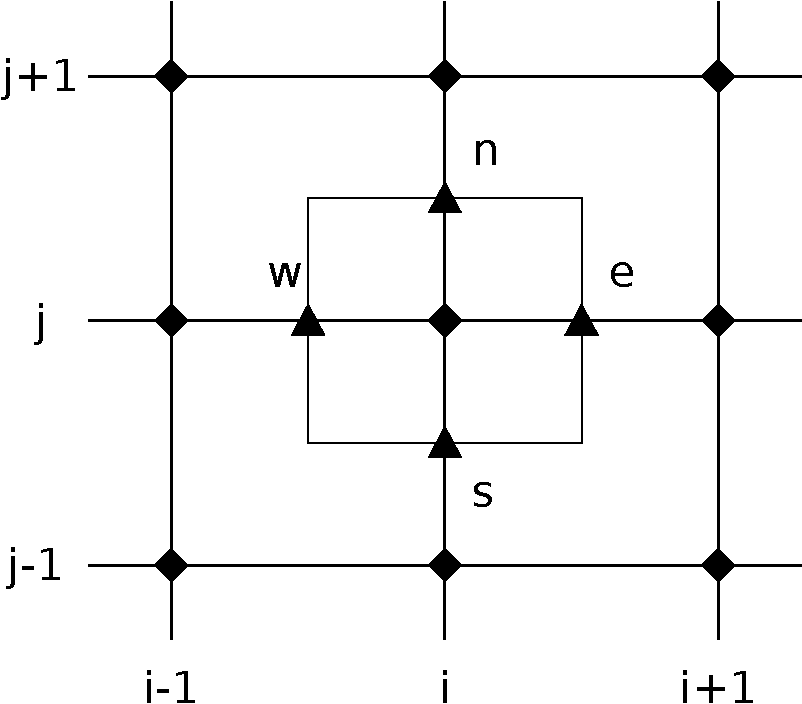
\includegraphics[width=2.0in,keepaspectratio=true]{figs/diffstencil}
\bigskip
\caption{Numerical scheme \eqref{eq:Wfd} for Equation \eqref{eq:adeqn} is a finite volume scheme for the grid-centered cell (dashed line).  The velocity and diffusivity are evaluated at the staggered grid locations (triangles).  The state functions $W,P$ live at the regular grid points (diamonds).}
\label{fig:stencil}
\end{figure}

Now we can state our scheme for equation \eqref{eq:adeqn}.  To set notation, suppose our rectangular computational domain has $M_x \times M_y$ gridpoints $(x_i,y_j)$ with uniform spacing $\Delta x,\Delta y$.  Let $\Wlij \approx W(t_l,x_i,y_j)$ and $\Plij \approx P(t_l,x_i,y_j)$ be the approximations of the continuum solution at the grid points.  Recall that $\Div \left(\bV W\right) = (\alpha W)_x + (\beta W)_y$.  We will compute velocity components at staggered (cell-face-centered) points as in Figure \ref{fig:stencil}.  We compute these values based on centered finite difference approximations of Equation \eqref{eq:vexpression}.  Let $c_0=K/(\rho_w g)$, a derived parameter used for convenience, so that $\bV = - c_0 \grad P - K \grad b$.  We use ``compass'' notation like $\alpha_e = \alpha_{i+1/2,j}$, and so on, for the components:
\begin{align}
\alpha_e &= - c_0 \frac{P_{i+1,j}-P_{i,j}}{\Delta x} - K \frac{b_{i+1,j}-b_{i,j}}{\Delta x}, \qquad \alpha_w = - c_0 \frac{P_{i,j}-P_{i-1,j}}{\Delta x} - K \frac{b_{i,j}-b_{i-1,j}}{\Delta x}, \label{eq:velocitycomp} \\
\beta_n  &= - c_0 \frac{P_{i,j+1}-P_{i,j}}{\Delta y} - K \frac{b_{i,j+1}-b_{i,j}}{\Delta y}, \qquad \beta_s = - c_0 \frac{P_{i,j}-P_{i,j-1}}{\Delta y} - K \frac{b_{i,j}-b_{i,j-1}}{\Delta y}. \notag
\end{align}
For the diffusive term the staggered-grid values are computed by averaging:
\begin{align}
W_e &= (W_{i,j}^l + W_{i+1,j}^l)/2, & W_w &= (W_{i-1,j}^l + W_{i,j}^l)/2, \label{eq:stagW} \\
W_n &= (W_{i,j}^l + W_{i,j+1}^l)/2, & W_s &= (W_{i,j-1}^l + W_{i,j}^l)/2. \notag
\end{align}

We apply the conservative upwind scheme in each variable, indicating the active index (either $i$ or $j$) in our upwind notation:
\begin{align}
 &\frac{W_{i,j}^{l+1} - \Wlij}{\Delta t} + \frac{\upp{\alpha_e}{\Wlij}{i} - \upp{\alpha_w}{W_{i-1,j}^l}{i}}{\Delta x} + \frac{\upp{\beta_n}{\Wlij}{j} - \upp{\beta_s}{W_{i,j-1}^l}{j}}{\Delta y}  \label{eq:Wfd} \\
      &\qquad = K \bigg[\frac{W_e \left(W_{i+1,j}^l - \Wlij\right) - W_w \left(\Wlij - W_{i-1,j}^l\right)}{\Delta x^2}  \notag \\
      &\qquad\qquad\qquad + \frac{W_n \left(W_{i,j+1}^l - \Wlij\right) - W_s \left(\Wlij - W_{i,j-1}^l\right)}{\Delta y^2}\bigg] + \Phi_{ij}. \notag
\end{align}
This scheme, which uses first-order upwinding, has $O(\Delta t^1 + \Delta x^1 + \Delta y^1)$ truncation error.

Because of the positivity proven in the appendix for this scheme, if $\Phi\ge 0$ then the lower bound $W\ge 0$ is true for the updated values at the new time $t_{l+1}$ if it is true at time $t_l$.  However, because refreeze is possible, generally $\Phi$ has either sign and so we must enforce $W\ge 0$ on the updated values.

\subsection*{Numerical scheme for pressure diffusion equation \eqref{eq:diffusionpressure}}  The pressure evolution equation is a nonlinear diffusion with additional ``reaction'' terms.  Unlike \eqref{eq:adeqn} there is no dominating advection term.  We discretize it using an explicit centered, second-order scheme.  Again, because this is an explicit scheme, we consider stable time steps immediately.

The time step restriction is comparable to \eqref{eq:dtDIFFW}, though the proof in the appendix does not suffice to \emph{prove} stability under this condition because of the additional reaction terms.  Noting that $P_o=\rho_i g H$, the time step must satisfy $\Delta t \le \Delta t_P$ where
\begin{equation}
\Delta t_P\, \left(\frac{2 K \rho_i \max H \max W}{\rho_w E_0}\right) \left(\frac{1}{\Delta x^2} + \frac{1}{\Delta y^2}\right) = \frac{1}{2} \label{eq:dtDIFFP}
\end{equation}

The resulting time step $\Delta t_P$ is a fraction of $\Delta t_W$ from \eqref{eq:dtDIFFW}:
\begin{equation}
\Delta t_P = \frac{\rho_w E_0}{\rho_i \max H}\, \Delta t_W.
\end{equation}
In fact, with the estimates $\rho_w/\rho_i \approx 1$, $E_0\approx 1$ m, and $\max H \approx 1000$ m we have $\Delta t_P$ which is about 1000 times smaller than $\Delta t_W$.  With these values and others used earlier (i.e.~$\Delta x = \Delta y = 500$ m, $\max |\bV|=10^5$ m/a, $K=10^{-2}$ m/s and $\max W=1$ m) we get
\begin{align*}
  \Delta t_{\text{CFL}} &\approx 0.001  \text{ year} &&\text{ from \eqref{eq:dtCFL}}, \\
  \Delta t_W            &\approx 0.1    \text{ year} &&\text{ from \eqref{eq:dtDIFFW}}, \\
  \Delta t_P            &\approx 0.0001 \text{ year} &&\text{ from \eqref{eq:dtDIFFP}.}
\end{align*}
Thus the numerical scheme for pressure diffusion, given next, has the shortest time step.  This analysis says if is only about 10 times shorter than the CFL restriction for the advection, however.  Furthermore, the precise size of the stable time step $\Delta t_P$ scales inversely with the adjustable small thickness $E_0$; by choosing $E_0$ larger we can make the time step restriction on $\Delta t_P$ less severe.

Now, the scheme we use for \eqref{eq:diffusionpressure} is similar to \eqref{eq:Wfd} for \eqref{eq:adeqn}:
\begin{align}
\frac{E_0}{(P_o)_{i,j}} \frac{P_{i,j}^{l+1} - \Plij}{\Delta t} &= c_0 \bigg[\frac{W_e \left(\psi_{i+1,j}^l - \psi_{i,j}^l\right) - W_w \left(\psi_{i,j}^l - \psi_{i-1,j}^l\right)}{\Delta x^2}  \label{eq:Pfd} \\
      &\qquad\qquad + \frac{W_n \left(\psi_{i,j+1}^l - \psi_{i,j}^l\right) - W_s \left(\psi_{i,j}^l - \psi_{i,j-1}^l\right)}{\Delta y^2}\bigg] \notag \\
      &\qquad + c_2 A \left(\rho_i g H_{i,j}- \Plij\right)^3 \Wlij - c_1 |\bv_b|_{i,j} \left(W_r - \Wlij\right)_+ + \Phi_{i,j}. \notag
\end{align}

Equation \eqref{eq:Pfd} is a reasonable statement of our scheme, but for implementation it is useful to have it in explicit update form.  First define
	$$\omega_x = \frac{c_0 \Delta t}{\Delta x^2}, \qquad \omega_y = \frac{c_0 \Delta t}{\Delta y^2}.$$
Also let
\newcommand{\Ocavij}{O_{\text{cav};\, i,j}}
\newcommand{\Ccrpij}{C_{\text{crp};\, i,j}}
	$$\Ocavij = c_1 |\bv_b|_{i,j} \left(W_r - \Wlij\right)_+, \qquad \Ccrpij = c_2 A \left(\rho_i g H_{i,j} - \Plij\right)^3 \Wlij$$
be the gridded values of the cavitation-opening and creep-closure rates.  Then scheme \eqref{eq:Pfd} is equivalent to this form:
\begin{align}
P_{i,j}^{l+1} &= \Plij +  \frac{(P_o)_{i,j}}{E_0} \bigg[\omega_x W_e \left(\psi_{i+1,j}^l - \psi_{i,j}^l\right) - \omega_x W_w \left(\psi_{i,j}^l - \psi_{i-1,j}^l\right) \label{eq:Pfdupdate} \\
      &\qquad\qquad\qquad\quad + \omega_y W_n \left(\psi_{i,j+1}^l - \psi_{i,j}^l\right) - \omega_y W_s \left(\psi_{i,j}^l - \psi_{i,j-1}^l\right) \notag \\
      &\qquad\qquad\qquad\quad + \Delta t\, \left(\Ccrpij - \Ocavij + \Phi_{i,j}\right)\bigg]. \notag
\end{align}

\subsection*{One time step of model \eqref{eq:bluebox}}  FIXME (THIS IS SKETCH):  Assume geometry fixed and thus $h_{i,j}$, $b_{i,j}$ and $(P_o)_{i,j}$ are determined for the duration of the run..  We start the step with values $\Wlij$, $\Plij$ which satisfy the bounds $W\ge 0$ and $0 \le P \le P_o$.  Get velocity components at staggered grid locations from \eqref{eq:velocitycomp}.  Get $W$ values averaged onto the staggered grid from \eqref{eq:stagW}.  Compute the current values of the hydraulic potential, $\psi_{i,j}^l = \Plij + \rho_w g(b_{i,j} + \Wlij)$.  Use \eqref{eq:Wfd} and \eqref{eq:Pfdupdate}.  Generally $\Phi$ has either sign and so we must enforce $W\ge 0$ on the updated values.  Thus, if $W_{i,j}^{l+1}<0$ at the end of a step we reset $W_{i,j}^{l+1}=0$.  The amount of mass created by this projection should be accounted for.  As the temporal grid is refined, however, this mass conservation error should decrease.  Alternatively we could redistribute mass to preserve exact conservation.  There is no expectation that pressure update \eqref{eq:Pfdupdate} will preserve our bounds $0\le P \le P_o$.  Thus, at the end of each pressure-update time step we \emph{project} to put the pressure $P_{i,j}^{l+1}$ back into this correct range.  Note that pressure is not a conserved quantity, so this projection step does not have accounting issues like that for the update to $W$.

\small
\bibliography{ice_bib}  % generally requires link to pism/doc/ice_bib.bib
\bibliographystyle{agu}
\normalsize

\appendix

\section{Positivity and stability of the numerical scheme for mass conservation}

Explicit numerical scheme \eqref{eq:Wfd} for the model PDE \eqref{eq:adeqn} is sufficiently simple so that we can analyze its properties.  The scheme is conditionally stable with conditions we give below.  We also note that the scheme is positivity-preserving: if the water input $\Phi$ is nonnegative and the discrete water thicknesses $\Wlij$ are also nonnegative at step $t_l$ then, under the stability conditions, the updated values $W_{i,j}^{l+1}$ are also nonnegative.  In this appendix we sketch a maximum principle argument \citep{MortonMayers} which shows both stability and the positivity-preserving property.

Let $\nu_x = \Delta t/\Delta x$, $\nu_y = \Delta t/\Delta y$, $\mu_x = K \Delta t / (\Delta x)^2$, and $\mu_y = K \Delta t / (\Delta y)^2$.  We consider only the case where all of the discrete velocities at the middle of the cell edges are nonnegative: $\alpha_e\ge 0$, $\alpha_w\ge 0$, $\beta_n\ge 0$, $\beta_s\ge 0$.  The many other cases, where these velocity components have various signs, can be handled by similar special-case arguments like the present one, and these other cases are left as a standard exercise for the reader \citep{MortonMayers}.

We rewrite \eqref{eq:Wfd} as a computation of the next value $W_{i,j}^{l+1}$, and collect terms:
\begin{align*}
 W_{i,j}^{l+1} &= \Wlij - \nu_x \left(\alpha_e \Wlij - \alpha_w W_{i-1,j}^l\right) - \nu_y \left(\beta_n \Wlij - \beta_s W_{i,j-1}^l\right)  \\
      &\qquad + \mu_x \left[W_e \left(W_{i+1,j}^l - \Wlij\right) - W_w \left(\Wlij - W_{i-1,j}^l\right)\right]  \\
      &\qquad + \mu_y \left[W_n \left(W_{i,j+1}^l - \Wlij\right) - W_s \left(\Wlij - W_{i,j-1}^l\right)\right] + \Delta t \Phi_{ij} \\
      &= (\nu_x \alpha_w + \mu_x W_w) W_{i-1,j}^l + (\mu_x W_e) W_{i+1,j}^l + (\nu_y \beta_s + \mu_y W_s) W_{i,j-1}^l + (\mu_y W_n) W_{i,j+1}^l \\
      &\qquad + \Big[1 - \nu_x \alpha_e - \nu_y \beta_n - \mu_x (W_e + W_w) - \mu_y (W_n + W_s)\Big] \Wlij + \Delta t \Phi_{ij}.
\end{align*}
The new value is a linear combination of the old values, plus a source term:
\begin{equation}
W_{i,j}^{l+1} = A W_{i-1,j}^l + B W_{i+1,j}^l + C W_{i,j-1}^l + D W_{i,j+1}^l + E \Wlij + \Delta t \Phi_{ij}. \label{eq:lincomb}
\end{equation}

Because of our assumption about nonnegative velocities, and assuming $\Wlij \ge 0$ for all $i,j$, coefficients $A,B,C,D$ are all nonnegative, and only $E$ could be negative, depending on the time step.  Thus we can state a sufficient condition based on an equal split between advective and diffusive parts.

Let us assume a CFL-type time step restriction for the advection term in  \eqref{eq:adeqn}:
\begin{equation}
\nu_x \alpha_e + \nu_y \beta_n = \Delta t \left(\frac{\alpha_e}{\Delta x} + \frac{\beta_n}{\Delta y}\right) \le \frac{1}{2}. \label{eq:adstabcond}
\end{equation}
Because we also handle the diffusion term in \eqref{eq:adeqn} explicitly, we have second time-step restriction:
\begin{equation}
\mu_x (W_e + W_w) + \mu_y (W_n + W_s) = \Delta t \left(\frac{K(W_e + W_w)}{\Delta x^2} + \frac{K(W_n + W_s)}{\Delta y^2}\right) \le \frac{1}{2}. \label{eq:diffstabcond}
\end{equation}
The right-hand sides of these inequalities are each $1/2$, but of course $1-(1/2)-(1/2)=0$.  In other words the coefficient $E$ in \eqref{eq:lincomb} is nonnegative:
	$$E = 1 - \nu_x \alpha_e - \nu_y \beta_n - \mu_x (W_e + W_w) - \mu_y (W_n + W_s) \ge 0.$$

Though the argument can only be made fully rigorous by handling all upwind cases (not shown), we see that all coefficients in linear combination \eqref{eq:lincomb} are nonnegative if the time step restrictions are satisfied.  Furthermore the coefficients add to one.  It follows \citep{MortonMayers} that scheme \eqref{eq:Wfd} is positivity-preserving when $\Phi\ge 0$, and it is stable under conditions \eqref{eq:adstabcond} and \eqref{eq:diffstabcond}.


\section{An alternative nearly-full closure}

A possible alternative to \eqref{eq:dampeddstrong}, which also replaces rigid constraint \eqref{eq:strongclosure} with a damped version, is described in this Appendix.

Choose a characteristic time scale $\tau$ which should be short (hours to months) compared to ice flow change time scales (months to centuries).  Consider this equation
\begin{equation}
- \tau \frac{\partial Y}{\partial t} = Y - W. \label{eq:dampedclosure}
\end{equation}
As $\tau \to 0$ this equation recovers the full-cavity closure $Y=W$.  It says that if the notional cavity upper surface ($Y$) is locally above the water level ($Y>W$) then it should lower ($\partial Y/\partial t < 0$), and, vice versa, if the notional cavity upper surface is locally below the water ($Y<W$) then the cavity top should rise ($\partial Y/\partial t > 0$).

Equation \eqref{eq:dampedclosure} does not allow us to eliminate $Y$, but it allows us to express pressure in terms of the geometric state variables $W$ and $Y$, as follows.  Solve \eqref{eq:capacity} for $N$, thus $P$, and substitute the expression for $\partial Y/\partial t$ from \eqref{eq:dampedclosure}:
\begin{equation}
P = P_o - \left(\frac{\tau^{-1} (Y-W) + c_1 |\bv_b| (W_r - Y)_+}{c_2 A Y}\right)^{1/3}.  \label{eq:pressurenormal}
\end{equation}

The above expression for $P$ applies only in certain ``normal'' cases, however.  In particular it assumes positive effective pressure ($N\ge 0 \iff P \le P_o$). The denominator of the fraction in \eqref{eq:pressurenormal} is always positive but the numerator
   $$\mathcal{Z} = \tau^{-1} (Y-W) + c_1 |\bv_b| (W_r - Y)_+$$
can change sign.  We have the following conditional scheme for pressure:
\begin{equation}
P = \begin{cases}
0, & \mathcal{Z} \ge c_2 A Y P_o^3, \\
P_o, & \mathcal{Z} \le 0, \\
P_o - \mathcal{Z}^{1/3} (c_2 A Y)^{-1/3}, & \text{all other cases}.
\end{cases} \label{eq:pressureWY}
\end{equation}
The last ``normal pressure'' case occurs exactly when formula \eqref{eq:pressurenormal} computes a pressure satisfying the bounds \eqref{eq:bounds}.

By \eqref{eq:pressureWY} we can compute pressure in terms of $Y,W$, namely $P = f(Y,W)$.   Thus, at each time step, we can start with the geometric data $h,b$ and the current values of the state variables $W,Y$ and we compute $P_o$, $\mathcal{Z}$, $P$, and $\bV$ in turn.  Then we update the state variables using the two evolution equations, which are equations \eqref{eq:adeqn} and \eqref{eq:dampedclosure}.

Equation \eqref{eq:dampedclosure} can be discretized by a semi-implicit (backward) first-order Euler method \citep{BurdenFaires}, assuming we have first computed the updated water thickness $W_{i,j}^{l+1}$ from \eqref{eq:Wfd}:
\begin{equation}
\frac{Y_{i,j}^{l+1} - Y_{i,j}^{l}}{\Delta t} = \frac{Y_{i,j}^{l+1} - W_{i,j}^{l+1}}{- \tau}. \label{eq:Yfd}
\end{equation}
This scheme is a very stable first-draft numerical scheme.  It can be rewritten as a direct calculation of the updated value,
   $$Y_{i,j}^{l+1} = \frac{1}{1 + (\Delta t/\tau)}\, Y_{i,j}^{l} + \frac{1}{1 + (\tau / \Delta t)}\, W_{i,j}^{l+1}.$$
Note $Y_{i,j}^{l+1}$ as a linear combination of $Y_{i,j}^{l}$ and $W_{i,j}^{l+1}$ with coefficients which are positive, less than one, and add to one.  Thus the scheme is unconditionally stable, at least when decoupled (i.e.~if the evolution of $W$ were not dependent on $Y$).

However, in all trial runs of this model a ``checkerboard'' instability of the pressure variable was observed, and sometimes of $W$ and/or $Y$.  The apparent reason for this instability is that the closure does not recover the effect of the highest-order term in the PDE \eqref{eq:ellipticpressure}, which is to say the elliptic part.  The diffusive closure in the main text has that part and it does not show evidence of any such instability.


\end{document}
